\documentclass[12pt]{article}

\usepackage{fullpage}
\usepackage{mathtools}
\usepackage{tikz}
\usepackage{caption}
\usepackage{subcaption}

\usepackage{csquotes}
\usepackage[backend=bibtex]{biblatex}
\addbibresource{node.dating}

\newcommand{\code}[1]{\emph{#1}}

\title{node.dating: methodology}

\author{Bradley R. Jones and Art F. Y. Poon}

\begin{document}
	\maketitle
	
	\section{General algorithm}	
		\code{node.dating} uses a tip to root maximum likelihood approach, based on \cite{Felsenstein81, TipDates}, to estimate the dates of the internal nodes of a phylogenetic tree given a rooted phylogenetic tree with branch length in number of molecular substitutions per base and dated tips.
		
		The mutation rate, $\mu$ of the tree is estimated by estimating the parameter $\mu$ in the linear model:
		\[\mathbf{D}_n = \mu\mathbf{t}_n + a,\]
		where $\mathbf{t}_n$ is the date of the tip, $n$, of the phylogenetic tree, $\mathbf{D}_n$ is the distance of $n$ from the root, in expected number of substitutions per base, and $a$ and $\mu$ are estimated parameters.
		The mutation rate can optionally be provided.
		
		Starting from the nodes furthest from the root (disregarding edge length), the date, $t^*$, of each node $n$ is chosen to maximize the product of the likelihoods, $\mathcal{L}_e(t_c - t^*)$, of its child edges (See Figure  \ref{fig:init}). For binary trees, we computed a closed form solution to likelihood optimization problem. If the tree is not binary, the \code{optimize} function of R is used instead.
		
		\begin{figure}[h]
			\centering
			\begin{subfigure}{.3\textwidth}
			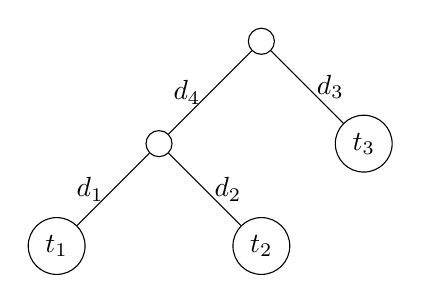
\begin{tikzpicture}[scale=1.3]
				\path (-2, -2) node[draw, circle] (n1){$t_1$}
				(0, -2) node[draw, circle] (n2){$t_2$}
				(1, -1) node[draw, circle] (n3){$t_3$}
				(-1, -1) node[draw, circle] (n4){}
				(0, 0) node[draw, circle] (n5){};
				
				\draw (n1) -- node[anchor=east] {$d_1$} (n4) -- node[anchor=east] {$d_4$} (n5) -- node[anchor=west] {$d_3$} (n3)
				(n4) -- node[anchor=west] {$d_2$} (n2);				
			\end{tikzpicture}
			\subcaption{}
			\end{subfigure}
			\begin{subfigure}{.3\textwidth}
			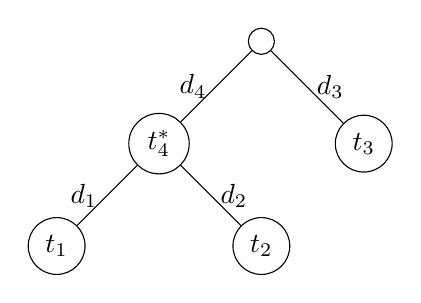
\begin{tikzpicture}[scale=1.3]
				\path (-2, -2) node[draw, circle] (n1){$t_1$}
				(0, -2) node[draw, circle] (n2){$t_2$}
				(1, -1) node[draw, circle] (n3){$t_3$}
				(-1, -1) node[draw, circle] (n4){$t_4^*$}
				(0, 0) node[draw, circle] (n5){};
				
				\draw (n1) -- node[anchor=east] {$d_1$} (n4) -- node[anchor=east] {$d_4$} (n5) -- node[anchor=west] {$d_3$} (n3)
				(n4) -- node[anchor=west] {$d_2$} (n2);				
			\end{tikzpicture}
			\subcaption{}
			\end{subfigure}
			\begin{subfigure}{.3\textwidth}
			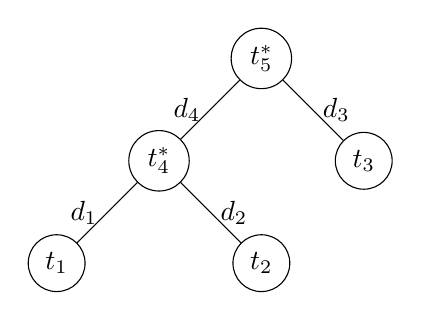
\begin{tikzpicture}[scale=1.3]
				\path (-2, -2) node[draw, circle] (n1){$t_1$}
				(0, -2) node[draw, circle] (n2){$t_2$}
				(1, -1) node[draw, circle] (n3){$t_3$}
				(-1, -1) node[draw, circle] (n4){$t_4^*$}
				(0, 0) node[draw, circle] (n5){$t_5^*$};
				
				\draw (n1) -- node[anchor=east] {$d_1$} (n4) -- node[anchor=east] {$d_4$} (n5) -- node[anchor=west] {$d_3$} (n3)
				(n4) -- node[anchor=west] {$d_2$} (n2);				
			\end{tikzpicture}
			\subcaption{}
			\end{subfigure}
			\caption{Initially the tree in (a) has edge lengths $d_1, \ldots, d_5$ (measured in substitutions per base) and times on the tips, $t_1$, $t_2$, and $t_3$ (measured in units of time). In the first step, the algorithm processes internal nodes in the order of distance from the root. First $t_4^*$ is chosen (b) to maximize the product of likelihoods of the node's child edges using times, $t_1$ and $t_2$, and edge lengths, $d_1$ and $d_2$. Next $t_5^*$ is chosen (c) to maximize the product of likelihoods of the node's child edges using times, $t_3$ and $t_4^*$, and edge lengths, $d_3$ and $d_4$.
			\label{fig:init}}
		\end{figure}
		
		Then the algorithm runs successive steps now choosing the date to maximize the product of the likelihoods of all of a node's edges (See Figure \ref{fig:step}). The algorithm runs a specified number of steps or until the difference in successive likelihoods of the tree is less than a specified threshold.

		\begin{figure}[h]
			\centering
			\begin{subfigure}{.3\textwidth}
			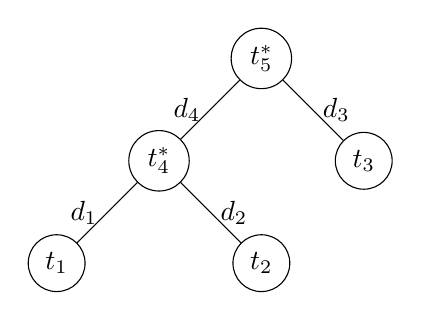
\begin{tikzpicture}[scale=1.3]
				\path (-2, -2) node[draw, circle] (n1){$t_1$}
				(0, -2) node[draw, circle] (n2){$t_2$}
				(1, -1) node[draw, circle] (n3){$t_3$}
				(-1, -1) node[draw, circle] (n4){$t_4^*$}
				(0, 0) node[draw, circle] (n5){$t_5^*$};
				
				\draw (n1) -- node[anchor=east] {$d_1$} (n4) -- node[anchor=east] {$d_4$} (n5) -- node[anchor=west] {$d_3$} (n3)
				(n4) -- node[anchor=west] {$d_2$} (n2);				
			\end{tikzpicture}
			\subcaption{}
			\end{subfigure}
			\begin{subfigure}{.3\textwidth}
			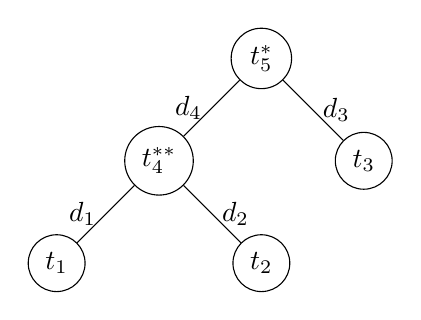
\begin{tikzpicture}[scale=1.3]
				\path (-2, -2) node[draw, circle] (n1){$t_1$}
				(0, -2) node[draw, circle] (n2){$t_2$}
				(1, -1) node[draw, circle] (n3){$t_3$}
				(-1, -1) node[draw, circle] (n4){$t_4^{**}$}
				(0, 0) node[draw, circle] (n5){$t_5^*$};
				
				\draw (n1) -- node[anchor=east] {$d_1$} (n4) -- node[anchor=east] {$d_4$} (n5) -- node[anchor=west] {$d_3$} (n3)
				(n4) -- node[anchor=west] {$d_2$} (n2);				
			\end{tikzpicture}
			\subcaption{}
			\end{subfigure}
			\begin{subfigure}{.3\textwidth}
			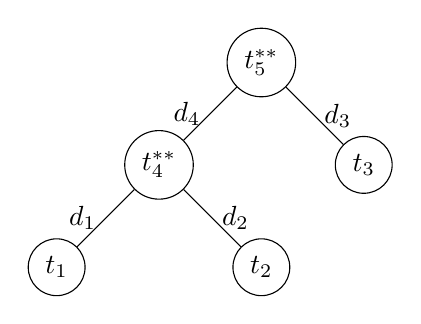
\begin{tikzpicture}[scale=1.3]
				\path (-2, -2) node[draw, circle] (n1){$t_1$}
				(0, -2) node[draw, circle] (n2){$t_2$}
				(1, -1) node[draw, circle] (n3){$t_3$}
				(-1, -1) node[draw, circle] (n4){$t_4^{**}$}
				(0, 0) node[draw, circle] (n5){$t_5^{**}$};
				
				\draw (n1) -- node[anchor=east] {$d_1$} (n4) -- node[anchor=east] {$d_4$} (n5) -- node[anchor=west] {$d_3$} (n3)
				(n4) -- node[anchor=west] {$d_2$} (n2);				
			\end{tikzpicture}
			\subcaption{}
			\end{subfigure}
			\caption{At the start, (a), of the second step of the algorithm the tree's internal nodes have times: $t_4^*$ and $t_5^*$.  Again, the algorithm processes internal nodes in the order of distance from the root. First $t_4^{**}$ is chosen (b) to maximize the product of likelihoods of the node's edges using times, $t_1$, $t_2$, and $t_5^*$, and edge lengths, $d_1$, $d_2$ and $d_4$. Next $t_5^{**}$ is chosen (c) to maximize the product of likelihoods of the node's child edges using times, $t_3$ and $t_4^{**}$, and edge lengths, $d_3$ and $d_4$.
			\label{fig:step}}
		\end{figure}	
	
	\section{Likelihood function}
		The likelihood of an assignment of dates, $\mathbf{t}$, to the nodes of a phylogenetic tree, $T$, is defined as the product of the likelihood of the edges:
		\[\mathcal{L}_T(\mathbf{t}) = \prod_{e \in E(T)}\mathcal{L}_e(\mathbf{t}_{c(e)} - \mathbf{t}_{p(e)}),\]
		where $p(e), c(e)$ are the parent and child nodes of the edge, $e$.
		The likelihood of an edge, $e$, is given by the gamma distribution:
		\[\mathcal{L}_e(t) = \operatorname{Gamma}(t; d(e) + 1, \mu) = \frac{{(d(e) + 1)}^{\mu}}{\Gamma(d(e) + 1)}t^{d(e)}e^{-\mu t},\]
		with $\mu$: the mutation rate and $d(e)$: the length of $e$.
		
		For efficiency, \code{node.dating}, uses the log likelihood instead of the likelihood to give:
		\[\log\mathcal{L}_e(t) = \mu\log d(e) - \log\Gamma(d(e) + 1) + d(e) \log t - \mu t,\]
		and the log likelihood of the tree is given by:
		\begin{align*}
			\log\mathcal{L}_T(t) = \sum_{e \in E(T)} & \big(\mu\log (d(e) + 1) - \log\Gamma(d(e) + 1) + \\
			&\qquad d(e) \log (t_{c(e)} - t_{p(e)}) - \mu (t_{c(e)} - t_{p(e)})\big). \\
		\end{align*}
		The summands $\mu\log (d(e) + 1)$ and $- \log\Gamma(d(e) + 1)$ are independent of $t$ and thus can be ignored when maximizing.
		
		In the case of binary trees calculus can be used to solve for the maximum likelihood.
		For binary trees, in the initial step and always at the root the function to be maximized is given by:
		\[f_n(t) = d(e_1) \log (t_1-t) - \mu (t_1 - t) + d(e_2) \log (t_2 - t) - \mu (t_2 - t),\]
		where $e_1, e_2$ are the edge lengths of the child edges and $t_1, t_2$ are the times of the children.
		It follows from calculus that in an interval $[a, b]$, a differentiable function, $f$, is maximized either at $f(a)$, $f(b)$ or at $f(c)$, where $f'(c) = 0$ or $f'(c)$ is undefined.
		The derivative of $f_n$ is given by:
		\[f_n'(t) = \frac{d(e_1)}{t-t_1} + \mu + \frac{d(e_2)}{t - t_1} + \mu.\]
		The solutions to $f_n'(t) = 0$ are equivalent to the solutions of the polynomial:
		\[2\mu t^2 + (d(e_1)+d(e_2)-2\mu (t_1+t_2))t + 2\mu t_1t_2-t_1d_2-t_2d_1=0.\]
		Solving this polynomial and comparing its solutions to the endpoints gives us our maximum.
		Similarly, for internal nodes in successive steps the function to be maximized is given by:
		\begin{align*}
			g_n(t) &= d(e_p) \log (t-t_p) - \mu (t-t_p) + \\
			&\qquad d(e_1) \log (t_1-t) - \mu (t_1 - t) + \\
			&\qquad d(e_2) \log (t_2 - t) - \mu (t_2 - t),
		\end{align*}
		where $d(e_1), d(e_2)$ are the edge lengths of the child edges, $t_1, t_2$ are the times of the children, $d(e_p))$ is the edge lengths of the parent edge, and $t_p$ is the last estimated time of the parent.
		Taking the derivative we get:
		\[g_n'(t) = \frac{d(e_1)}{t-t_p} - \mu + \frac{d(e_1)}{t-t_1} + \mu + \frac{d(e_2)}{t - t_1} + \mu.\]
		The solutions to $g_n'(t) = 0$ are equivalent to the solutions of the polynomial:
		\begin{align*}
			&\mu t^3+ \\
			&\qquad \big(d(e_p) + d(e_1) + d(e_2) - \mu(t_p + t_1 + t_2)\big) t^2 + \\
			&\qquad \big(\mu (t_pt_1 + t_pt_2 + t_1t_2) - (t_1 + t_2) d(e_p) - (t_p + t_2) d(e_1) - (t_p + t_1) d(e_p)\big) t +  \\
			&\qquad d(e_p)t_1t_2 + d(e_1)t_pt_2 + d(e_2)t_1t_p - \mu t_p t_1 t_2 = 0.
		\end{align*}
		Again, solving this polynomial and comparing its solutions to the endpoints gives us our maximum.
	\printbibliography{}
\end{document}